%%%%%%%%%%%%%%%%%%%%%%%%%%%%%%%%%%%%%%%%%%%%%%%%%%%%%%%%%%%%%%%%%%%%%%%
% Slides for the TechCon 2022 talk "PyAnsys Tools for Unit Testing" 
%%%%%%%%%%%%%%%%%%%%%%%%%%%%%%%%%%%%%%%%%%%%%%%%%%%%%%%%%%%%%%%%%%%%%%%
\documentclass[t]{beamer}

\usetheme{Ansys2022}

\usepackage{minted}
\usepackage{xcolor}
\usepackage{pdfpages}
\usepackage{listings}
\usepackage{tikz}
\usepackage{hyperref}

\usepackage[edges]{forest}
\hypersetup{
    colorlinks=true,
    linkcolor=blue,
    filecolor=magenta,      
    urlcolor=cyan,
}
 

\urlstyle{same}
\setbeamercolor{background canvas}{bg=}

\definecolor{bleudefrance}{rgb}{0.19, 0.55, 0.91}

%%%%%%%%%%%%%%%%%%%%%%%%%%%%%%%%%%%%%%%%%%%%%%%%%%%%%%%%%%%%%%%%%%%%%%%%%%%%%%%
\usetikzlibrary{shapes.geometric, arrows,positioning}

\tikzset{
  startstop/.style={
    rectangle, 
    rounded corners,
    minimum width=3cm,
    minimum height=0.75cm,
    align=center, 
    draw=black, 
    fill=ANSYS@Gold,
    },
  process/.style={
    rectangle, 
    minimum width=3cm, 
    minimum height=0.75cm, 
    align=center, 
    draw=black, 
    fill=ANSYS@Blue,
    text=white,
    },
  decision/.style={
    diamond, 
    aspect=4,
    minimum width=3cm, 
    minimum height=1cm,
    align=center,
    draw=black, 
    fill=ANSYS@Blue,
    text=white,
    },
  arrow/.style={thick,->,>=stealth},
  dec/.style={
    ellipse, 
    align=center, 
    draw=black, 
    fill=ANSYS@Bronze,
    },
}

\begin{document}

%%%%%%%%%%%%%%%%%%%%%%%%%%%%%%%%%%%%%%%%%%%%%%%%%%%%%%%%%%%%%%%%%%%%%%%%%%%%%%%
%% Title Slide

\title{pytest - Framework for Unit Testing}
\subtitle{\small Applying test-driven development within Ansys}
\author{Alex Kaszynski \\ Jorge Martinez Garrido}
\date{\today}

\titleframe{}


%%%%%%%%%%%%%%%%%%%%%%%%%%%%%%%%%%%%%%%%%%%%%%%%%%%%%%%%%%%%%%%%%%%%%%%%%%%%%%%
%% Table of contents

\begin{frame}{Table of Contents}
  \tableofcontents
  \vspace{200pt}  %% force top left  
\end{frame}


%%%%%%%%%%%%%%%%%%%%%%%%%%%%%%%%%%%%%%%%%%%%%%%%%%%%%%%%%%%%%%%%%%%%%%%%%%%%%%%
\transitionframe{Introduction}
\section{Introduction}

%%%%%%%%%%%%%%%%%%%%%%%%%%%%%%%%%%%%%%%%%%%%%%%%%%%%%%%%%%%%%%%%%%%%%%%%%%%%%%%
\begin{frame}[fragile=singleslide]
  \frametitle{Introduction}

  \vspace{-15pt}

  \begin{itemize}
  \setlength\itemsep{1em}

  \item{\textbf{What is test-driven development (TDD)?}
    \\Software requirements are converted to test cases before software is
    fully developed.
    \\As soon as the code base gets modified, a collection of tests get executed
    to guarantee the integrity of the new code.
  }

  \item{\textbf{What are its main advantages?}
    \begin{itemize}
    \item \small Improved design of the system.
    \item \small Better code quality and flexibility.
    \item \small Good documentation as a byproduct.
    \item \small Lower development costs and increased developer productivity.
    \end{itemize}
  }
  
  \vspace{-3pt}
  \item {\textbf{\href{https://pytest.org/}{pytest} is a and powerful and mature testing framework widely used in Python.}
    }

  \end{itemize}

\end{frame}

%%%%%%%%%%%%%%%%%%%%%%%%%%%%%%%%%%%%%%%%%%%%%%%%%%%%%%%%%%%%%%%%%%%%%%%%%%%%%%%
%%%%%%%%%%%%%%%%%%%%%%%%%%%%%%%%%%%%%%%%%%%%%%%%%%%%%%%%%%%%%%%%%%%%%%%%%%%%%%%
\begin{frame}[fragile=singleslide]
  \frametitle{Test Driven Development - Overview}
  \vspace{-10pt}
  \centering
  \href{https://en.wikipedia.org/wiki/Test-driven_development}{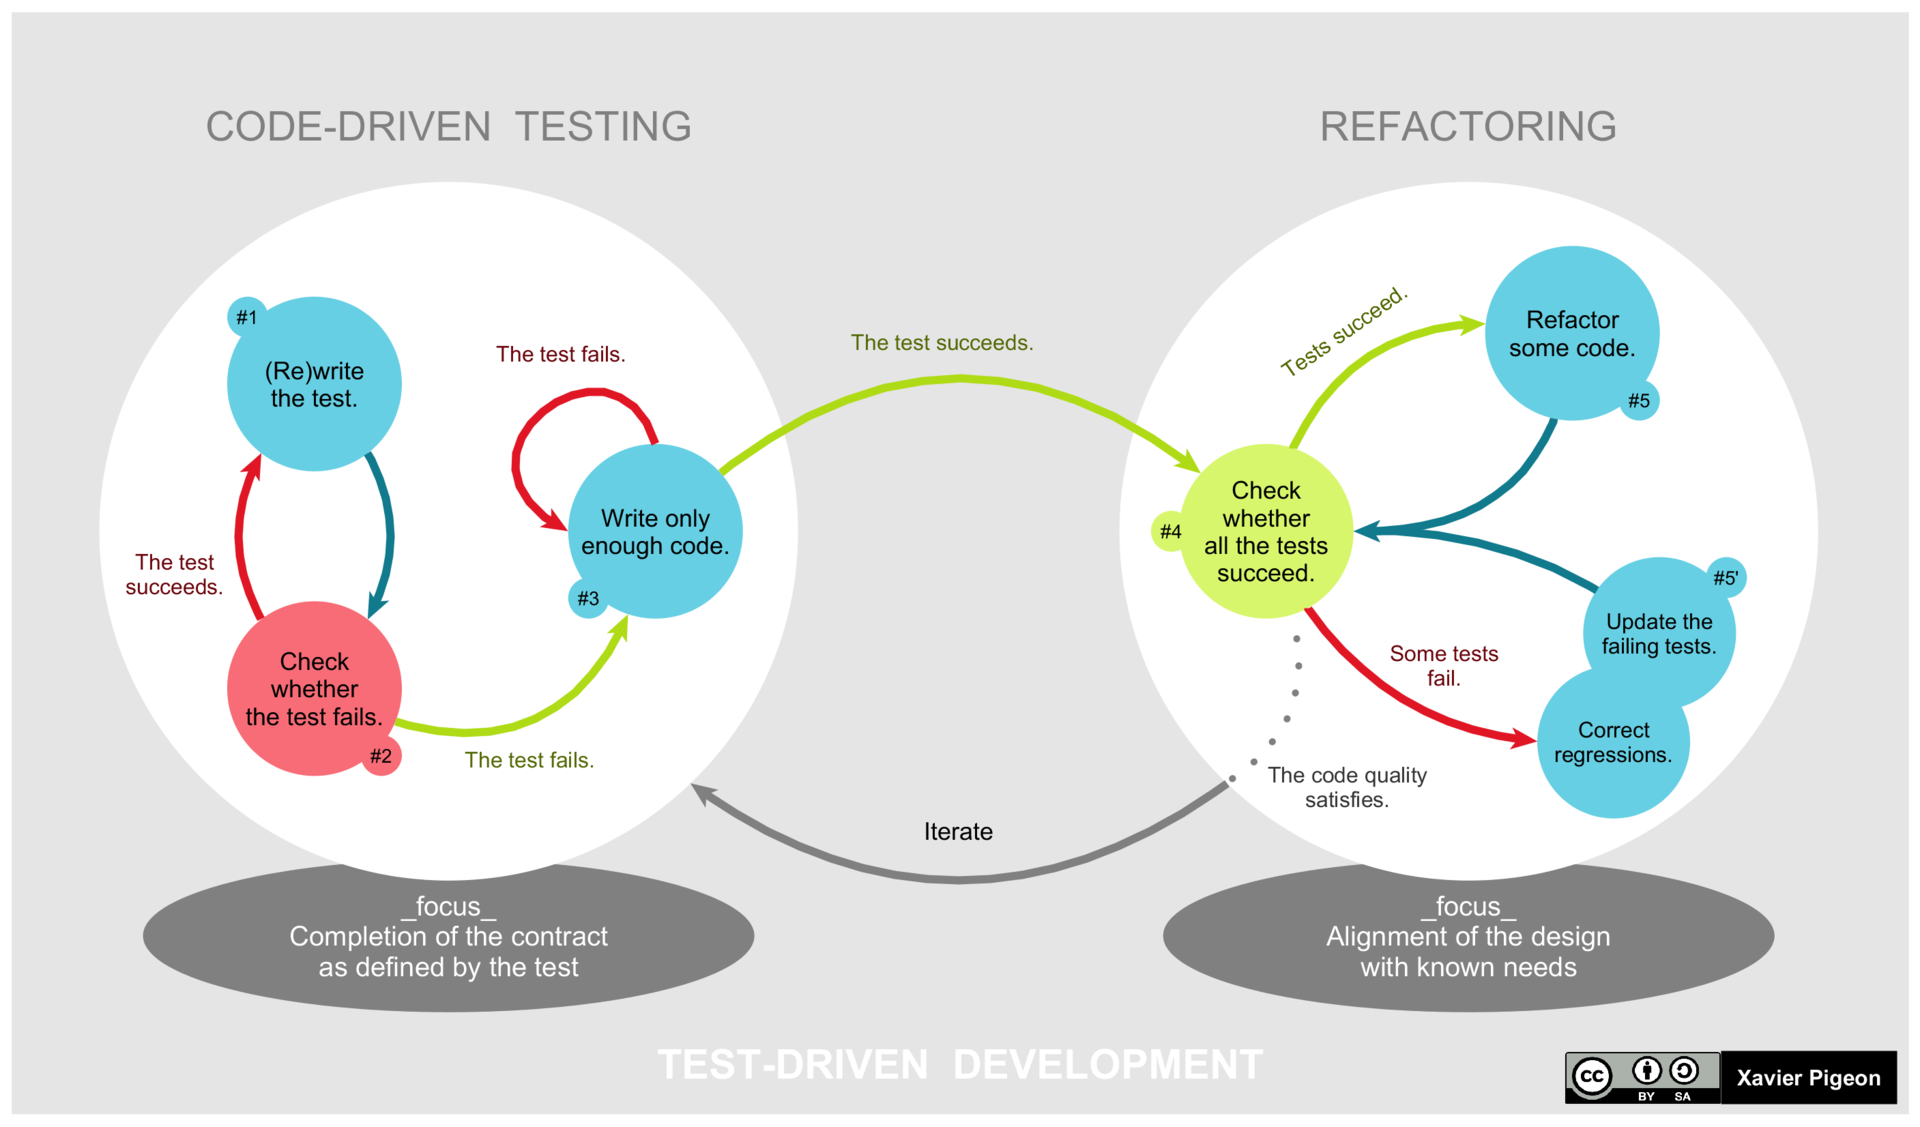
\includegraphics[width=0.8\textwidth]{figures/1920px-TDD_Global_Lifecycle.png}}

  %% By Xarawn - Own work, CC BY-SA 4.0, https://commons.wikimedia.org/w/index.php?curid=44782343

\end{frame}



%%%%%%%%%%%%%%%%%%%%%%%%%%%%%%%%%%%%%%%%%%%%%%%%%%%%%%%%%%%%%%%%%%%%%%%%%%%%%%%
\transitionframe{Overview of pytest}
\section{Overview of pytest}

\begin{frame}
  \frametitle{Content}
  \tableofcontents[currentsection]
  \vspace{200pt}  %% force top left
\end{frame}


%%%%%%%%%%%%%%%%%%%%%%%%%%%%%%%%%%%%%%%%%%%%%%%%%%%%%%%%%%%%%%%%%%%%%%%%%%%%%%%
\subsection{Basic assertions with pytest}
\begin{frame}[fragile=singleslide]
  \frametitle{Basic assertions with pytest}

   \begin{itemize}
   \item Tests are defined using functions starting with \texttt{test}
   \item Use the \href{https://docs.python.org/3/reference/simple_stmts.html#the-assert-statement}{assert} statement to compare current and expected results.
   \item Run your tests by invoking \href{https://docs.pytest.org/en/7.1.x/how-to/usage.html}{pytest}.
   \end{itemize}

  \begin{columns}[T]
    \begin{column}{.5\textwidth}
      \begin{exampleblock}{Basic Assertion}
        \inputminted[fontsize=\footnotesize]{python}{code/basic_assertion.py}
      \end{exampleblock}
    \end{column}

    \begin{column}{.5\textwidth}
      \centering
      \href{https://asciinema.org/a/535234}{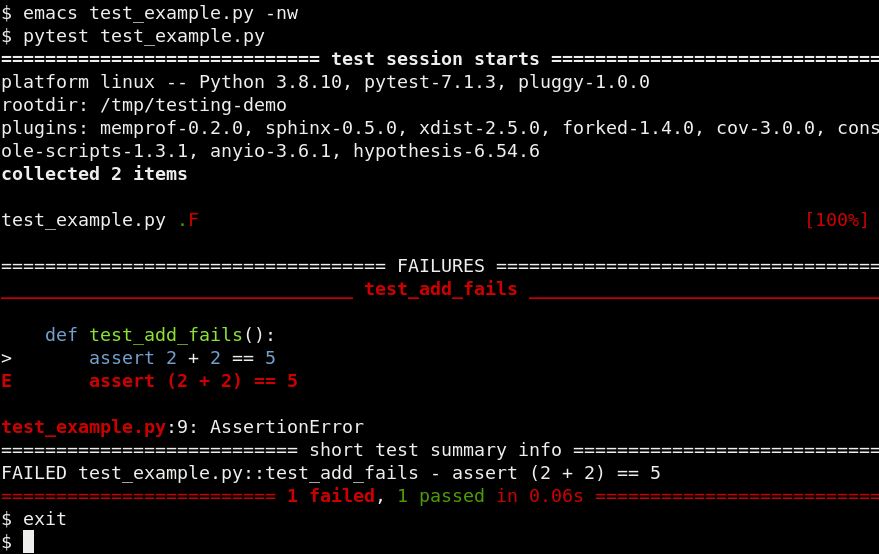
\includegraphics[width=0.9\textwidth]{figures/pytest_simple.png}}
    \end{column}
  \end{columns}

\end{frame}

%%%%%%%%%%%%%%%%%%%%%%%%%%%%%%%%%%%%%%%%%%%%%%%%%%%%%%%%%%%%%%%%%%%%%%%%%%%%%%%
\subsection{Array assertions}
\begin{frame}[fragile=singleslide]
  \frametitle{Using NumPy for Floating Point Assertions}

   \begin{itemize}
        \item For floating point values, absolute and relative tolerances are required.
        \item \href{https://numpy.org/doc/stable/index.html}{NumPy} provides the \href{https://numpy.org/doc/stable/reference/generated/numpy.testing.assert_allclose.html}{assert\_allclose} function for this purpose.
        \item You can also use \href{https://numpy.org/doc/stable/reference/generated/numpy.testing.assert_equal.html}{assert\_equal} to check if two arrays are exactly the same.
   \end{itemize}

  \begin{columns}[T]
    \begin{column}{.5\textwidth}
      \vspace{-5pt}
      \begin{exampleblock}{\small Array Assertions}
        \inputminted[fontsize=\scriptsize]{python}{code/float_assertion.py}
      \end{exampleblock}
    \end{column}

    \begin{column}{.5\textwidth}
      \centering
      \href{https://asciinema.org/a/535241}{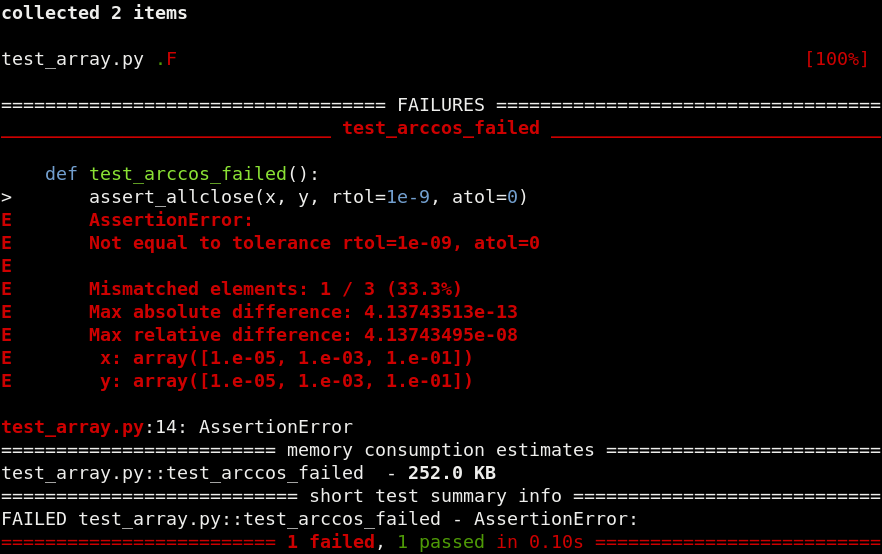
\includegraphics[width=0.9\textwidth]{figures/pytest_array.png}}
    \end{column}
  \end{columns}

\end{frame}

%%%%%%%%%%%%%%%%%%%%%%%%%%%%%%%%%%%%%%%%%%%%%%%%%%%%%%%%%%%%%%%%%%%%%%%%%%%%%%%
\subsection{Marking tests}
\begin{frame}[fragile=singleslide]
  \frametitle{Marking Tests}

   \begin{itemize}
       \item Marking tests allows to filter and select desired tests from the test suite.
       \item Marking is performed using the \texttt{pytest.mark.<name>} decorator.
       \item Select marked tests by executing \texttt{pytest -m <name> -vv tests}
   \end{itemize}

  \begin{columns}[T]
    \begin{column}{.5\textwidth}
      \vspace{-5pt}
      \begin{exampleblock}{\small \texttt{pytest.mark.<name>}}
        \inputminted[fontsize=\scriptsize]{python}{code/marked_test.py}
      \end{exampleblock}
    \end{column}

    \begin{column}{.5\textwidth}
      \centering
      \href{https://asciinema.org/a/535244}{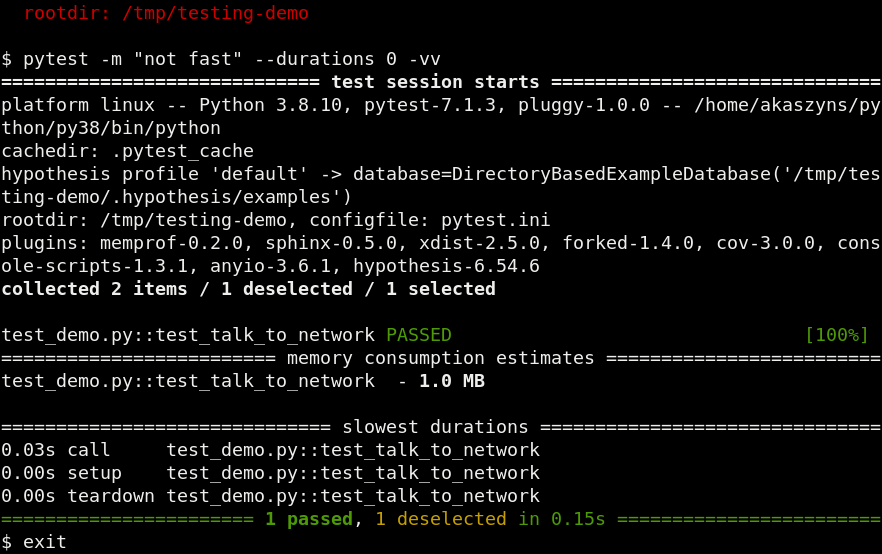
\includegraphics[width=0.9\textwidth]{figures/pytest_mark.png}}
    \end{column}
  \end{columns}

\end{frame}


%%%%%%%%%%%%%%%%%%%%%%%%%%%%%%%%%%%%%%%%%%%%%%%%%%%%%%%%%%%%%%%%%%%%%%%%%%%%%%%
\subsection{Parameterizing tests}
\begin{frame}[fragile=singleslide]
  \frametitle{Parametrizing tests}

   \begin{itemize}
   \item Parameterizing a allows you to run the same test with different
     inputs.
   \item This allows you to reuse test code and test a variety of inputs.
   \item Using the
     \href{https://docs.pytest.org/en/6.2.x/parametrize.html}{pytest.mark.parametrize}
     decorator.
   \end{itemize}

  \begin{columns}[T]
    \begin{column}{.5\textwidth}
      \vspace{-5pt}
      \begin{exampleblock}{\small \texttt{pytest.mark.parametrize}}
        \inputminted[fontsize=\scriptsize]{python}{code/parametrized_test.py}
      \end{exampleblock}
    \end{column}

    \begin{column}{.5\textwidth}
      \centering
      \href{https://asciinema.org/a/535248}{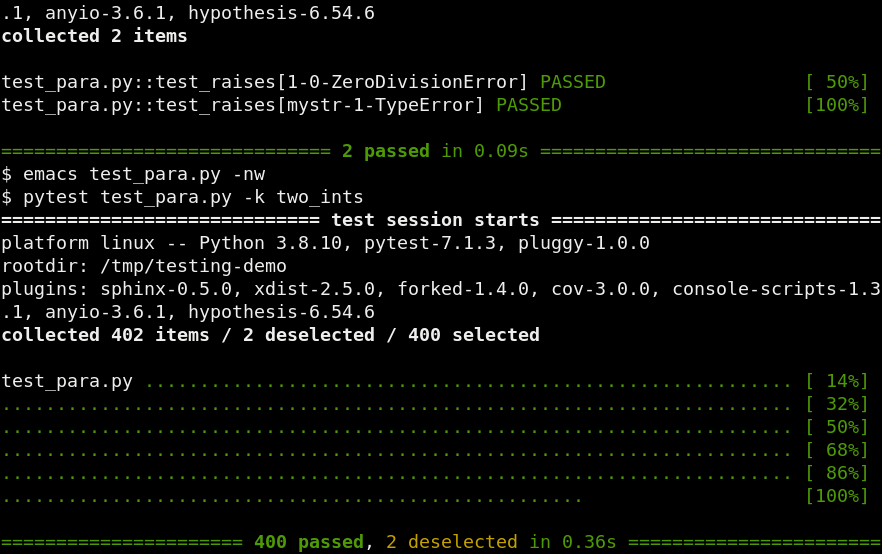
\includegraphics[width=0.9\textwidth]{figures/pytest_para.png}}
    \end{column}
  \end{columns}

\end{frame}



%%%%%%%%%%%%%%%%%%%%%%%%%%%%%%%%%%%%%%%%%%%%%%%%%%%%%%%%%%%%%%%%%%%%%%%%%%%%%%%
\subsection{Plugins}
\begin{frame}[fragile=singleslide]
  \frametitle{A plethora of plugins}

   Plugins add or modify the behavior of \texttt{pytest}:

   \begin{exampleblock}{\small pytest-xdist}
     \vspace{-5pt}
     \begin{lstlisting}[basicstyle=\ttfamily\scriptsize]
$ pip install pytest-xdist
$ pytest -n auto
     \end{lstlisting}
     \vspace{-5pt}
   \end{exampleblock}

   \vspace{-3pt}

   \begin{itemize}
   \item \texttt{pytest} integrates with the
     \href{https://docs.python.org/3/library/unittest.html}{unittest} module
     from \href{https://docs.python.org/3/library/}{Python Standard Library}.
   \item Validate documentation examples with \href{https://docs.python.org/3/library/doctest.html}{doctests}.
   \item Check code coverage with \href{https://pypi.org/project/pytest-cov/}{pytest-cov}
   \item Include \href{https://matplotlib.org/}{Matplotlib} testing with \href{https://pypi.org/project/pytest-mpl/}{pytest-mpl}
   \item Find edge cases with \href{https://pypi.org/project/hypothesis/}{hypothesis}
   \end{itemize}

   \vspace{0.2em}

   Check out the official list at \href{https://docs.pytest.org/en/latest/reference/plugin\_list.html}{pytest - Plugin List}.

\end{frame}

%%%%%%%%%%%%%%%%%%%%%%%%%%%%%%%%%%%%%%%%%%%%%%%%%%%%%%%%%%%%%%%%%%%%%%%%%%%%%%%
\subsection{Continuous integration and development}
\begin{frame}[fragile=singleslide]
  \frametitle{Continuous integration and development}

  \vspace{-11pt}

  \begin{columns}[T]
    \begin{column}{.55\textwidth}
      \begin{itemize}
      \item At Ansys, Continuous integration and development (CI/CD) takes place in
        ADO or GitHub.
      \item It is performed using workflow and configured via YAML files and you can test across a variety of environments using a \href{https://docs.github.com/en/actions/using-jobs/using-a-matrix-for-your-jobs}{matrix} workflow.
      \item Automate testing using \texttt{pytest} across multiple OSes and platforms.
      \item Integrate with other third party apps like \href{https://app.codecov.io/gh/pyansys/pymapdl}{codecov} to provide metrics and insights.
      \end{itemize}
    \end{column}

    \begin{column}{.5\textwidth}
      \centering
      \href{https://github.com/pyansys/pymapdl/actions}{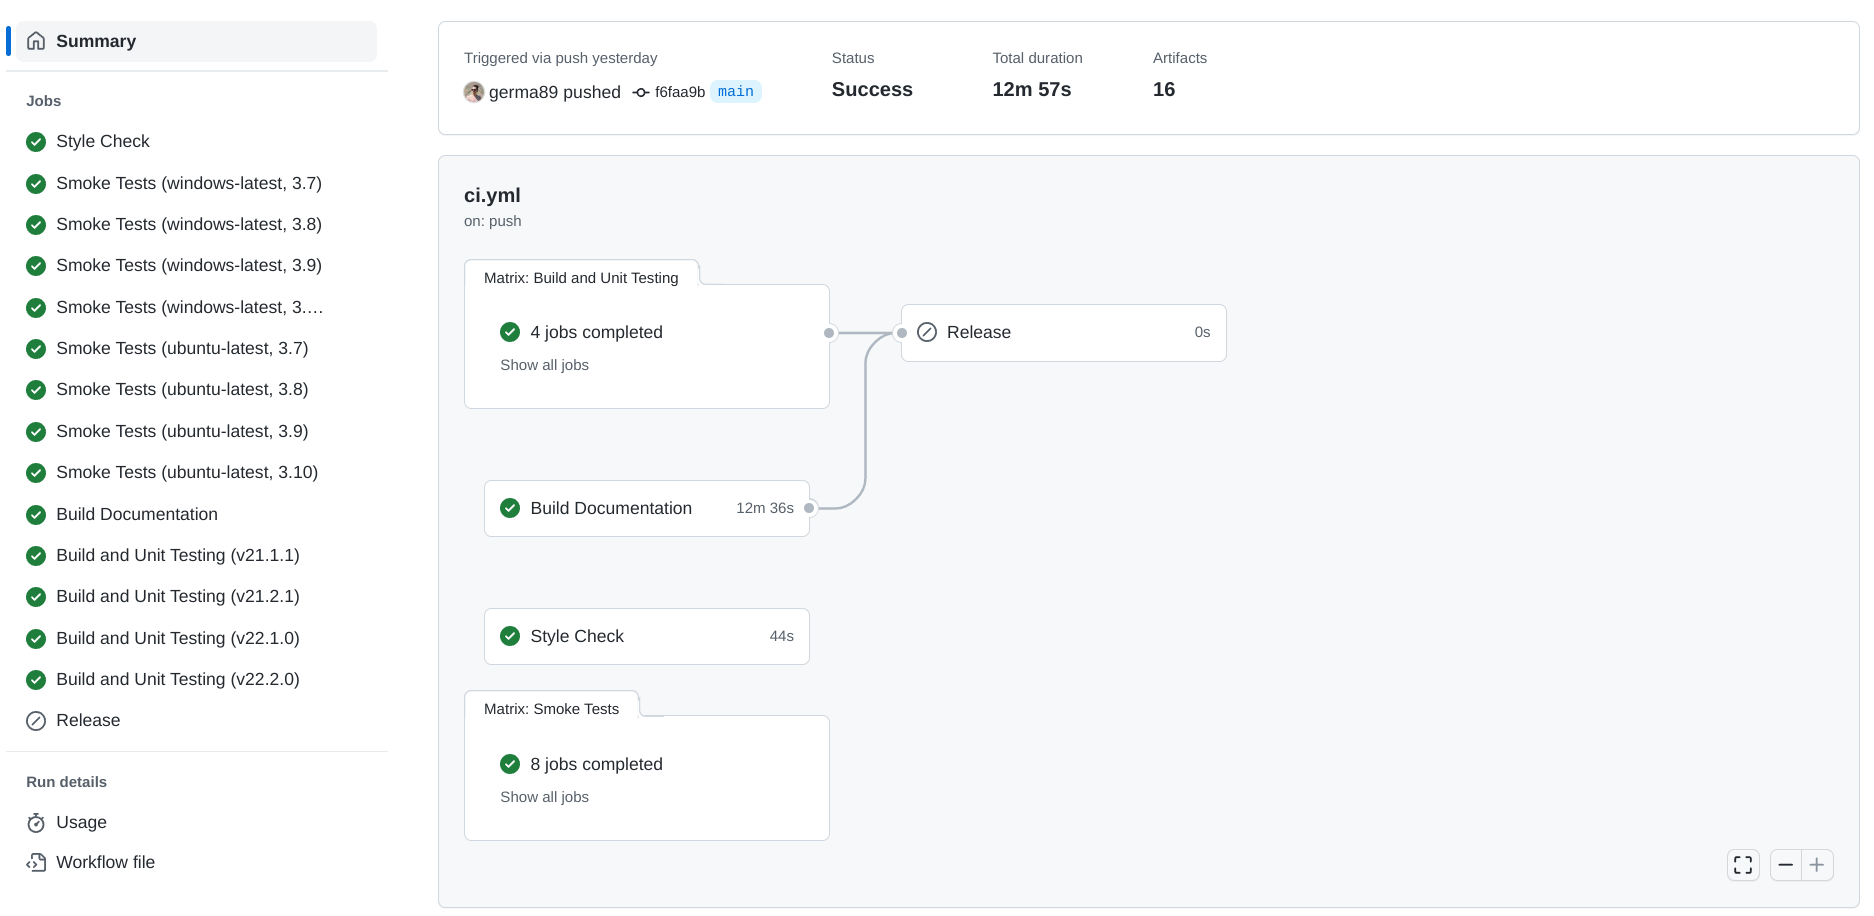
\includegraphics[width=1.0\textwidth]{figures/gh_actions_pipeline.png}}
      \begin{exampleblock}{\small workflow.yaml}
        \inputminted[fontsize=\scriptsize]{yaml}{code/workflow.yml}
      \end{exampleblock}

    \end{column}
  \end{columns}

\end{frame}


%%%%%%%%%%%%%%%%%%%%%%%%%%%%%%%%%%%%%%%%%%%%%%%%%%%%%%%%%%%%%%%%%%%%%%%%%%%%%%%
\section{Where to find help}
\transitionframe{Where to find help}

\begin{frame}
  \frametitle{Content}
  \tableofcontents[currentsection]
  \vspace{200pt}  %% force top left
\end{frame}

\begin{frame}[fragile=singleslide]
  \frametitle{Additional Information}

  Visit the \href{https://dev.docs.pyansys.com/}{PyAnsys Developer’s Guide} for
  more information on how to implement testing.

  %% \vspace{1em}
  \centering

  \vspace{1em}
  \textbf{PyAnsys Dev Guide - testing}
  \\\href{https://dev.docs.pyansys.com/how-to/testing.html}{https://dev.docs.pyansys.com/how-to/testing.html}

  \vspace{1em}
  \textbf{PyAnsys Dev Guide - Continuous Integration}
  \\\href{https://dev.docs.pyansys.com/how-to/continuous-integration.html}{https://dev.docs.pyansys.com/how-to/continuous-integration.html}

  \vspace{1em}
  \textbf{pytest - Documentation}
  \\\href{https://docs.pytest.org/en/latest/}{https://docs.pytest.org/en/latest/}

\end{frame}


\lastframe{}
\end{document}
